% Chapter 9 -- Symmetric matrices and the spectral theorem
\chapter{Symmetric matrices and the spectral theorem}\label{ch:spectral}

Symmetric matrices are the best-behaved class in all of linear algebra:
every eigenvalue is real, eigenvectors for different eigenvalues are
perpendicular, and there is always a full orthonormal eigenbasis. The
spectral theorem says a symmetric matrix is a rotation, an axis-aligned
stretch, and a rotation back. Everything downstream uses this --- PCA's
principal axes, the Hessian's curvature readout, quadratic-program
convexity, and the SVD's construction next chapter. After this chapter
you can diagonalise any symmetric matrix with an orthogonal $Q$,
classify definiteness three ways, use the Rayleigh quotient as a variational
eigenvalue finder, and read a covariance matrix geometrically.

% from-zero:begin
\begin{rulebox}[Before you start]
Chapters~5 and~7. \emph{Recap:} a matrix is \emph{symmetric} if $A=A^{\mathsf T}$. Covariance matrices, Hessians and $A^{\mathsf T}A$ are all symmetric, which is why this class matters so much.
\end{rulebox}
\begin{wins}[After this chapter you can]
\begin{itemize}
\item diagonalise a symmetric matrix with an orthonormal basis (the spectral theorem);
\item decide whether a quadratic form is positive definite;
\item use the Rayleigh quotient to find the largest and smallest eigenvalues;
\item explain why every covariance matrix is positive semidefinite.
\end{itemize}
\end{wins}
\begin{principle}[How to think about this]
Symmetric matrices behave beautifully: their eigenvectors are perpendicular, so the matrix is just independent stretching along perpendicular axes. That is why they appear whenever there is a notion of energy, curvature or spread. When you meet a symmetric matrix, think ``ellipse with perpendicular axes.''
\end{principle}
% from-zero:end

\section{Symmetric matrices and why they are special}\label{sec:sym-special}

\begin{definition}[Symmetric matrix]\index{symmetric matrix}
$A$ is \emph{symmetric} when $A^{T}=A$: entry $(i,j)$ equals entry
$(j,i)$. The Gram matrix $A^{T}A$, every covariance matrix, and every
Hessian of a smooth function are symmetric by construction.
\end{definition}

Two miracles happen for real symmetric matrices, proved in
Section~\ref{sec:handderiv9}:

\begin{theorem}[Real eigenvalues]\index{eigenvalue!real}
If $A=A^{T}$ is real, every eigenvalue of $A$ is real.
\end{theorem}

\begin{theorem}[Orthogonal eigenvectors]\index{eigenvector!orthogonality}
If $A=A^{T}$, eigenvectors belonging to \emph{distinct} eigenvalues are
orthogonal.
\end{theorem}

Neither holds in general: the rotation
$\begin{bmatrix}0&-1\\1&0\end{bmatrix}$ has eigenvalues $\pm i$
(chapter 7) --- symmetry is what removes complex eigenvalues and skew
eigenframes at once.

\section{The spectral theorem}\label{sec:spectral}

\begin{theorem}[Spectral theorem]\index{spectral theorem}
Every real symmetric $n\times n$ matrix factors as
\[
A=Q\Lambda Q^{T},
\]
where $Q$ is orthogonal ($Q^{T}Q=I$, columns = orthonormal eigenvectors)
and $\Lambda=\operatorname{diag}(\lambda_1,\dots,\lambda_n)$ is real.
\end{theorem}

Compare chapter 7: there $A=V\Lambda V^{-1}$ held only with a possibly
ill-conditioned $V$. Symmetry upgrades the basis change:
$V^{-1}$ becomes $Q^{T}$, perfectly conditioned and free.
Figure~\ref{fig:rotstretch} shows the geometry: rotate, stretch,
rotate back.

\begin{figure}[htbp]
\centering
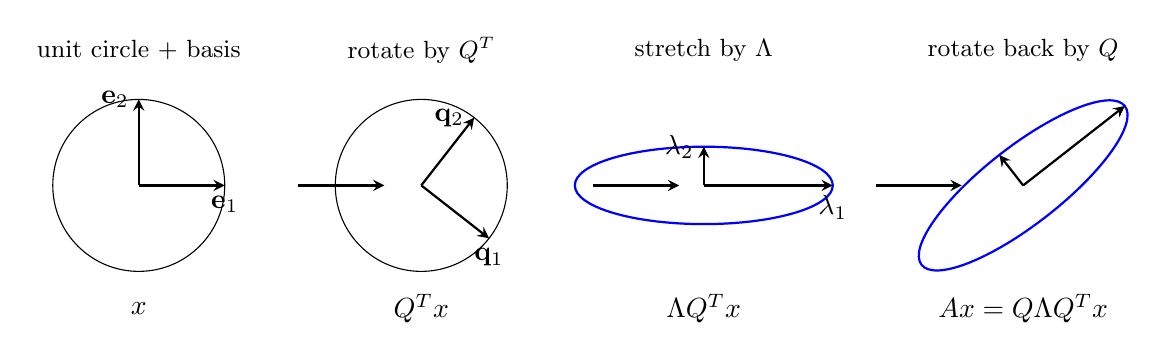
\begin{tikzpicture}[scale=0.78,>=stealth]
\node at (0,2.2) {\small unit circle + basis};
\draw (0,0) circle (1.4);
\draw[->,thick] (0,0)--(1.4,0) node[below]{$\mathbf e_1$};
\draw[->,thick] (0,0)--(0,1.4) node[left]{$\mathbf e_2$};
\node at (0,-2.0) {$x$};
\begin{scope}[xshift=4.6cm]
\node at (0,2.2) {\small rotate by $Q^{T}$};
\begin{scope}[rotate=-38]
\draw (0,0) circle (1.4);
\draw[->,thick] (0,0)--(1.4,0) node[below]{$\mathbf q_1$};
\draw[->,thick] (0,0)--(0,1.4) node[left]{$\mathbf q_2$};
\end{scope}
\node at (0,-2.0) {$Q^{T}x$};
\end{scope}
\begin{scope}[xshift=9.2cm]
\node at (0,2.2) {\small stretch by $\Lambda$};
\draw[blue,thick] (0,0) ellipse (2.1 and 0.63);
\draw[->,thick] (0,0)--(2.1,0) node[below]{$\lambda_1$};
\draw[->,thick] (0,0)--(0,0.63) node[left]{$\lambda_2$};
\node at (0,-2.0) {$\Lambda Q^{T}x$};
\end{scope}
\begin{scope}[xshift=14.4cm]
\node at (0,2.2) {\small rotate back by $Q$};
\begin{scope}[rotate=38]
\draw[blue,thick] (0,0) ellipse (2.1 and 0.63);
\draw[->,thick] (0,0)--(2.1,0);
\draw[->,thick] (0,0)--(0,0.63);
\end{scope}
\node at (0,-2.0) {$Ax=Q\Lambda Q^{T}x$};
\end{scope}
\foreach \xx in {2.6,7.4,12.0} \draw[->,thick] (\xx,0)--(\xx+1.4,0);
\end{tikzpicture}

\caption{$A=Q\Lambda Q^{T}$ geometrically: rotate into the eigenbasis,
stretch each axis by $\lambda_i$, rotate back. Notice there are no skew
angles anywhere --- unlike general diagonalisation, everything stays
orthogonal. Regenerate: \ttfamily figures/ch09\_rotstretch.tex.}
\label{fig:rotstretch}
\end{figure}

\begin{example}[Spectral decomposition by hand]\label{ex:spec2}
\textbf{Strategy.} For $A=\begin{bmatrix}2&1\\1&2\end{bmatrix}$ the
eigenvectors must come out orthonormal --- verify, then assemble
$Q\Lambda Q^{T}$.

\textbf{Solution.} $\chi_A=(2-\lambda)^2-1=\lambda^2-4\lambda+3$: roots
$\lambda_1=3$, $\lambda_2=1$. Eigenvectors: $(1,1)/\sqrt2$ for 3,
$(1,-1)/\sqrt2$ for 1 --- note $\langle(1,1),(1,-1)\rangle=0$ as promised.
Then
\[
A=\frac1{\sqrt2}\begin{bmatrix}1&1\\1&-1\end{bmatrix}
\begin{bmatrix}3&0\\0&1\end{bmatrix}
\frac1{\sqrt2}\begin{bmatrix}1&1\\1&-1\end{bmatrix}=Q\Lambda Q^{T}.
\]
Check the (1,1) entry: $\frac12(3\cdot1+1\cdot1)=2$ \checkmark.
\end{example}

\begin{lstlisting}[caption={\ttfamily code/ch09\_spec\_verify.py --- a random
symmetric matrix: eigenvalues real, $Q$ orthogonal, reconstruction exact.}]
import numpy as np
np.set_printoptions(precision=4, suppress=True)
rng = np.random.default_rng(3)

M = rng.standard_normal((4, 4))
A = M + M.T          # symmetric by construction
print("A ="); print(A)
print("symmetric:", np.allclose(A, A.T))

w, Q = np.linalg.eigh(A)   # eig for symmetric matrices
print("eigenvalues:", w)
print("Q orthonormal (Q^T Q = I):", np.allclose(Q.T @ Q, np.eye(4)))
Lam = np.diag(w)
print("A == Q Lambda Q^T:", np.allclose(Q @ Lam @ Q.T, A))
print("A^3 == Q Lambda^3 Q^T:",
      np.allclose(Q @ np.diag(w**3) @ Q.T, A @ A @ A))
# non-symmetric contrast: same eigenvalues? no orthogonal basis
B = np.array([[0., -1.], [1., 0.]])
print("rotation eig:", np.linalg.eigvals(B), "(complex: not symmetric)")
\end{lstlisting}

\begin{lstlisting}[caption={Output of the spectral check. Notice
\texttt{eigh} (the symmetric specialist) returns all-real eigenvalues and
a $Q$ that is orthonormal to machine precision --- and powers collapse to
$\Lambda^{k}$.}]
A =
[[ 4.0818 -3.0083 -0.4471 -0.8491]
 [-3.0083 -0.4312  1.303  -0.9   ]
 [-0.4471  1.303   0.4516 -1.4078]
 [-0.8491 -0.9     -1.4078 -0.7816]]
symmetric: True
eigenvalues: [-2.6815 -1.6239  1.8538  5.7722]
Q orthonormal (Q^T Q = I): True
A == Q Lambda Q^T: True
A^3 == Q Lambda^3 Q^T: True
rotation eig: [0.+1.j 0.-1.j] (complex: not symmetric)
\end{lstlisting}

\begin{exercise}[easy]
Decompose $\begin{bmatrix}3&0\\0&1\end{bmatrix}$ and
$\begin{bmatrix}1&2\\2&1\end{bmatrix}$ as $Q\Lambda Q^{T}$.
\begin{solution}
First is already $\Lambda$ with $Q=I$. Second: eigenvalues $3,-1$ with
$(1,1)/\sqrt2,(1,-1)/\sqrt2$ --- $Q$ orthogonal as required even though an
eigenvalue is negative (symmetric $\ne$ positive definite!).
\end{solution}
\end{exercise}

\section{Quadratic forms and definiteness}\label{sec:quadform}

\begin{definition}[Quadratic form]\index{quadratic form}
For symmetric $A$, $q(\mathbf x)=\mathbf x^{T}A\mathbf x$ is a pure
second-degree scalar --- a paraboloid, saddle, or degenerate sheet whose
level sets Figure~\ref{fig:levelsets} draws.
\end{definition}

\begin{definition}[Definiteness]\index{positive definite}\index{indefinite}
$A$ is \emph{positive definite} (PD) when $\mathbf x^{T}A\mathbf x>0$ for
all $\mathbf x\ne\mathbf0$; \emph{positive semidefinite} (PSD) when
$\ge0$; \emph{indefinite} when the form takes both signs. Negative
definite/semidefinite mirror with $\le,<0$.
\end{definition}

Three equivalent tests (each earns its keep):

\begin{center}
\begin{tabularx}{\textwidth}{l>{\raggedright\arraybackslash}X}
\toprule
\textbf{Test} & \textbf{Statement}\\
\midrule
Eigenvalues & PD iff every $\lambda_i>0$; PSD iff $\lambda_i\ge0$;
indefinite iff mixed signs \\
Pivots (Sylvester) & PD iff every pivot in elimination is positive ---
no eigenvalues needed \\
Leading minors & PD iff all leading principal minors $>0$ \\
\bottomrule
\end{tabularx}
\end{center}

\begin{example}[Classifying three ways]\label{ex:definite}
\textbf{Strategy.} Take the tridiagonal
$B=\begin{bmatrix}2&-1&0\\-1&2&-1\\0&-1&2\end{bmatrix}$ and classify by
pivots (cheap) then eigenvalues (decisive).

\textbf{Solution.} Elimination gives pivots $2,\ \tfrac32,\ \tfrac43$ ---
all positive, so $B$ is PD without touching eigenvalues. The listing
confirms: eigenvalues $0.586,2,3.414$ all positive. Contrast
$\begin{bmatrix}1&2\\2&1\end{bmatrix}$: eigenvalues $-1,3$ and pivots
$1,-3$ --- indefinite, its level sets are hyperbolas.
\end{example}

\begin{figure}[htbp]
\centering
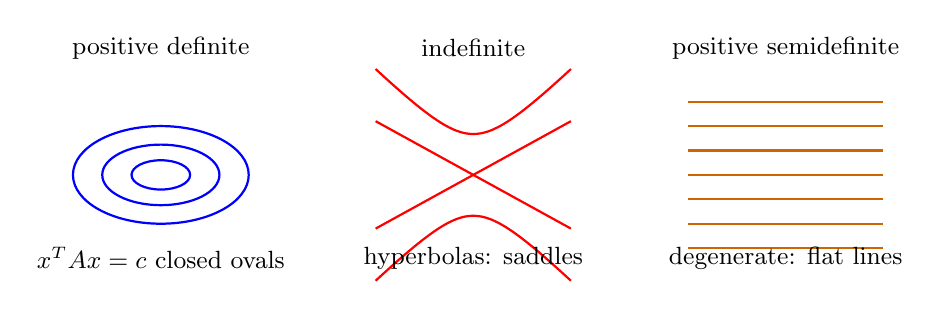
\begin{tikzpicture}[scale=0.62,>=stealth]
% PD: ellipses; INDEF: hyperbolas; PSD: parallel lines
\begin{scope}
\node at (0,2.6) {\small positive definite};
\draw[blue,thick] (0,0) ellipse (1.8 and 1.0);
\draw[blue,thick] (0,0) ellipse (1.2 and 0.62);
\draw[blue,thick] (0,0) ellipse (0.6 and 0.3);
\node at (0,-1.7) {\small $x^{T}Ax=c$ closed ovals};
\end{scope}
\begin{scope}[xshift=6.4cm]
\node at (0,2.6) {\small indefinite};
\draw[red,thick,domain=-2:2,smooth] plot (\x,{sqrt(0.7+\x*\x)});
\draw[red,thick,domain=-2:2,smooth] plot (\x,{-sqrt(0.7+\x*\x)});
\draw[red,thick,domain=-2:2,smooth] plot (\x,{0.55*\x});
\draw[red,thick,domain=-2:2,smooth] plot (\x,{-0.55*\x});
\node at (0,-1.7) {\small hyperbolas: saddles};
\end{scope}
\begin{scope}[xshift=12.8cm]
\node at (0,2.6) {\small positive semidefinite};
\foreach \y in {-1.5,-1.0,-0.5,0,0.5,1.0,1.5} \draw[orange!80!black,thick] (-2,\y)--(2,\y);
\node at (0,-1.7) {\small degenerate: flat lines};
\end{scope}
\end{tikzpicture}

\caption{Level sets $x^{T}Ax=c$ by definiteness. Notice positive definite
gives closed ellipses (a bowl), indefinite gives hyperbolas (a saddle),
semidefinite degenerates into parallel lines (a trough).
Regenerate: \ttfamily figures/ch09\_levelsets.tex.}
\label{fig:levelsets}
\end{figure}

\begin{lstlisting}[caption={\ttfamily code/ch09\_definiteness.py ---
eigenvalues vs.\ pivot signs on four matrices, then $A^{T}A$ is always
PSD.}]
import numpy as np
np.set_printoptions(precision=4, suppress=True)

def pivots(A):
    A = A.astype(float).copy(); n = A.shape[0]; ps = []
    for j in range(n):
        ps.append(A[j, j])
        if abs(A[j, j]) < 1e-12: break
        A[j+1:, j:] -= np.outer(A[j+1:, j] / A[j, j], A[j, j:])
    return np.array(ps)

mats = {
    "PD   [[2,-1,0],[-1,2,-1],[0,-1,2]]":
        np.array([[2., -1., 0.], [-1., 2., -1.], [0., -1., 2.]]),
    "PSD  [[1,1,1],[1,1,1],[1,1,1]]":
        np.ones((3, 3)),
    "IND  [[1,0],[0,-1]]":
        np.array([[1., 0.], [0., -1.]]),
    "PD?  [[1,2],[2,1]]":
        np.array([[1., 2.], [2., 1.]]),
}
for name, M in mats.items():
    w = np.linalg.eigvalsh(M)
    print(f"{name}: eigs {w}  pivots {pivots(M)}")

# A^T A is always PSD
rng = np.random.default_rng(0)
A = rng.standard_normal((5, 3))
G = A.T @ A
print("Gram G=A^T A eigenvalues:", np.linalg.eigvalsh(G))
x = rng.standard_normal(3)
print("x^T G x = ||Ax||^2 =", x @ G @ x, " = ||Ax||^2 check:",
      np.isclose(x @ G @ x, (A @ x) @ (A @ x)))
\end{lstlisting}

\begin{lstlisting}[caption={Output of the definiteness tests. Notice
pivots and eigenvalues agree in sign pattern on every case --- and the
Gram matrix's eigenvalues are all $\ge0$ because $x^{T}Gx=\lVert
Ax\rVert^{2}$ is a squared length, never negative.}]
PD   [[2,-1,0],[-1,2,-1],[0,-1,2]]: eigs [0.5858 2.     3.4142]  pivots [2.     1.5    1.3333]
PSD  [[1,1,1],[1,1,1],[1,1,1]]: eigs [-0. -0.  3.]  pivots [1. 0.]
IND  [[1,0],[0,-1]]: eigs [-1.  1.]  pivots [ 1. -1.]
PD?  [[1,2],[2,1]]: eigs [-1.  3.]  pivots [ 1. -3.]
Gram G=A^T A eigenvalues: [0.1121 2.9218 9.9282]
x^T G x = ||Ax||^2 = 8.095346091200302  = ||Ax||^2 check: True
\end{lstlisting}

\begin{proposition}[$A^{T}A$ is always PSD]
For any real $A$ (any shape),
$\mathbf x^{T}(A^{T}A)\mathbf x=\lVert A\mathbf x\rVert^{2}\ge0$. It is PD
exactly when $A$ has full column rank.
\end{proposition}

\begin{exercise}[medium]
Show $A$ PD $\Rightarrow$ $A$ invertible and $A^{-1}$ PD.
\begin{solution}
$\lambda_i>0$ means none is zero, so $\det A=\prod\lambda_i>0$ and
$A^{-1}=Q\Lambda^{-1}Q^{T}$ has eigenvalues $1/\lambda_i>0$ --- PD.
\end{solution}
\end{exercise}

\begin{example}[A semidefinite trap]\label{ex:psdtrap}
Is $A=\begin{bmatrix}1&2\\2&4\end{bmatrix}$ positive definite?
\par\smallskip
\textbf{Strategy.} Definiteness asks about \emph{every} $\mathbf{x}$:
$x^{T}Ax>0$. Check the eigenvalues --- and, for a fast counterexample
hunt, note that $\det A$ decides already: a $2\times2$ PD matrix has
positive determinant.
\begin{solution}
$\det A=4-4=0$, so $A$ is singular: $\lambda_2=0$ --- semidefinite,
not definite. Find the flat direction directly:
$A(2,-1)=(0,0)$, so $(2,-1)^{T}A(2,-1)=0$ exactly --- the trough of
figure~\ref{fig:defgallery}. Eigenvalues $0,5$ confirm: PSD with a
zero eigen-direction. \checkmark\ Moral: ``positive'' and ``positive
\emph{semi}definite'' differ by exactly the flat directions --- and
data matrices live there constantly.
\end{solution}
\end{example}

\begin{figure}[htbp]\centering
% Figure 9.x: definiteness read off level sets.
% x^T A x tells the story: bowl (PD), dome (ND), saddle (indef), trough (semi).
\begin{tikzpicture}[scale=0.72,>=stealth]
  % PD: concentric ellipses
  \begin{scope}
    \draw[thick,accent] (0,0) ellipse (0.5 and 0.28);
    \draw[thick,accent] (0,0) ellipse (0.95 and 0.55);
    \draw[thick,accent] (0,0) ellipse (1.4 and 0.82);
    \node[font=\footnotesize,align=center] at (0,-1.25) {positive definite\\ bowl, min at 0};
  \end{scope}
  % ND
  \begin{scope}[xshift=3.4cm]
    \draw[thick] (0,0) ellipse (0.5 and 0.28);
    \draw[thick] (0,0) ellipse (0.95 and 0.55);
    \draw[thick] (0,0) ellipse (1.4 and 0.82);
    \node[font=\footnotesize,align=center] at (0,-1.25) {negative definite\\ dome, max at 0};
  \end{scope}
  % indefinite: hyperbola
  \begin{scope}[xshift=6.8cm]
    \draw[thick,accent] plot[domain=-1.1:1.1] (\x,{0.4*\x*\x+0.15});
    \draw[thick,accent] plot[domain=-1.1:1.1] (\x,{-0.4*\x*\x-0.15});
    \draw[thick] plot[domain=-1.4:-0.3] (\x,{0.25/\x});
    \draw[thick] plot[domain=0.3:1.4] (\x,{0.25/\x});
    \draw[thick] plot[domain=-1.4:-0.3] (\x,{-0.25/\x});
    \draw[thick] plot[domain=0.3:1.4] (\x,{-0.25/\x});
    \node[font=\footnotesize,align=center] at (0,-1.25) {indefinite\\ saddle};
  \end{scope}
  % semidef: parallel lines (trough)
  \begin{scope}[xshift=10.2cm]
    \draw[thick,accent] (-1.3,0.55) -- (1.3,0.55);
    \draw[thick,accent] (-1.3,-0.55) -- (1.3,-0.55);
    \draw[thick] (-1.3,1.0) -- (1.3,1.0);
    \draw[thick] (-1.3,-1.0) -- (1.3,-1.0);
    \node[font=\footnotesize,align=center] at (0,-1.5) {semidefinite\\ trough: flat in the\\ zero-eigen direction};
  \end{scope}
\end{tikzpicture}

\caption{Definiteness by level sets. Notice the semidefinite case has
a \emph{flat} direction --- the zero eigenvalue --- where the form
stays $0$ no matter how far you walk.}
\label{fig:defgallery}
\end{figure}

\section{Rayleigh quotient}\label{sec:rayleigh}

\begin{definition}[Rayleigh quotient]\index{Rayleigh quotient}
For symmetric $A$ and $\mathbf x\ne\mathbf0$,
$R(\mathbf x)=\dfrac{\mathbf x^{T}A\mathbf x}{\mathbf x^{T}\mathbf x}$.
\end{definition}

Decompose $\mathbf x$ in the eigenbasis: $R$ is a weighted average of the
$\lambda_i$ with weights $c_i^{2}$ --- so it lives in
$[\lambda_{\min},\lambda_{\max}]$, and

\begin{theorem}[Min--max principle]\index{min-max principle}
$\max_{\mathbf x\ne\mathbf0}R(\mathbf x)=\lambda_1$ at $\mathbf x=\mathbf q_1$;
$\min_{\mathbf x\ne\mathbf0}R(\mathbf x)=\lambda_n$ at $\mathbf x=\mathbf q_n$.
The $k$-th eigenvalue is the max of $R$ over vectors orthogonal to
$\mathbf q_1,\dots,\mathbf q_{k-1}$.
\end{theorem}

This is why power iteration (chapter 7) converged to $\lambda_1$: it is
hill-climbing $R$ (Figure~\ref{fig:rayleigh}). It is also why PCA's first
component is a Rayleigh maximization --- Section~\ref{sec:covar}.

\begin{figure}[htbp]
\centering
\begin{tikzpicture}[scale=0.8,>=stealth]
% landscape: R(x) on unit circle, min/max at eigenvectors
\draw[->] (-2.6,0)--(2.6,0) node[right]{$x_1$};
\draw[->] (0,-2.6)--(0,2.6) node[above]{$x_2$};
\draw (0,0) circle (2.2);
\foreach \r in {0.6,1.1,1.6,2.1} \draw[blue!60,rotate=25] (0,0) ellipse ({\r*1.7} and {\r*0.55});
\draw[->,thick,red] (0,0)--({2.2*cos(25)},{2.2*sin(25)}) node[right=2pt]{$\mathbf q_1$: $R=\lambda_1$};
\draw[->,thick,red] (0,0)--({-2.2*sin(25)},{2.2*cos(25)}) node[above=2pt]{$\mathbf q_2$: $R=\lambda_2$};
\node at (0,-3.1) {$R(x)=\dfrac{x^{T}Ax}{x^{T}x}$ extremized at eigenvectors};
\end{tikzpicture}

\caption{$R(x)$ on the unit circle. Notice the quotient is maximized
along $\mathbf q_1$ and minimized along $\mathbf q_2$ --- the
eigenvectors are exactly the stationary directions of the landscape.
Regenerate: \ttfamily figures/ch09\_rayleigh.tex.}
\label{fig:rayleigh}
\end{figure}

\begin{exercise}[hard]
From the weighted-average picture, prove: if $\mathbf x$ is a stationary
point of $R$, then $\mathbf x$ is an eigenvector. (Hint: the gradient of
$R$ is proportional to $A\mathbf x-R(\mathbf x)\mathbf x$.)
\begin{solution}
$\nabla R=2(A\mathbf x-R\mathbf x)/\mathbf x^{T}\mathbf x$; stationary
$\Rightarrow$ $A\mathbf x=R\mathbf x$ --- the eigen equation with
$\lambda=R(\mathbf x)$.
\end{solution}
\end{exercise}

\begin{example}[Rayleigh quotient hands-on]\label{ex:rayq}
For $A=\begin{bmatrix}2&1\\1&2\end{bmatrix}$ (eigenvalues $3$ and $1$),
evaluate the Rayleigh quotient
$R(\mathbf{x})=\mathbf{x}^{T}A\mathbf{x}/\mathbf{x}^{T}\mathbf{x}$ on
$\mathbf{x}=(1,1)$, $(1,-1)$, and $(1,0)$ --- and confirm it never
leaves $[\lambda_{\min},\lambda_{\max}]$.
\par\smallskip
\textbf{Strategy.} The quotient is the stretch $A$ applies along a
direction, weighted by the eigenbasis mix. Test the two eigenvectors
first --- they must return the eigenvalues exactly.
\begin{solution}
$(1,1)$ is the $\lambda=3$ eigenvector: $A(1,1)=(3,3)$,
$R=6/2=3$. $(1,-1)$ gives $A(1,-1)=(1,-1)$, $R=2/2=1$. And
$(1,0)$: $A(1,0)=(2,1)$, $R=2/1=2$ --- between the eigenvalues,
since $(1,0)=\tfrac12(1,1)+\tfrac12(1,-1)$ mixes both directions.
\checkmark\ The quotients sweep $[1,3]$ as the direction turns ---
the whole machine behind both $\lambda_{\max}=\max R$ and the
power-iteration picture.
\end{solution}
\end{example}

\section{Covariance matrices: PSD by data}\label{sec:covar}

Center data matrix $X$ ($n$ rows of observations, $d$ feature columns)
and form $C=X^{T}X/(n-1)$. As a Gram matrix it is automatically PSD ---
and its eigenstructure IS the data's geometry:

\begin{example}[Covariance eigendecomposition]\label{ex:covspec}
\textbf{Strategy.} Build correlated 2-D data ($x_2=0.8x_1+\text{noise}$),
compute $C$, and read its eigenvalues/eigenvectors as the axes of the
data's spread --- a PCA preview.

\textbf{Solution.} The listing's $C=\begin{bmatrix}1.03&0.86\\0.86&0.88\end{bmatrix}$
has eigenvalues $1.82,0.09$: one direction carries $95\%$ of variance.
Its eigenvector $(-0.74,-0.68)$ is the long axis of the data ellipse
(Figure~\ref{fig:covellipse}) --- principal component 1, found by nothing
but the spectral theorem.
\end{example}

\begin{figure}[htbp]
\centering
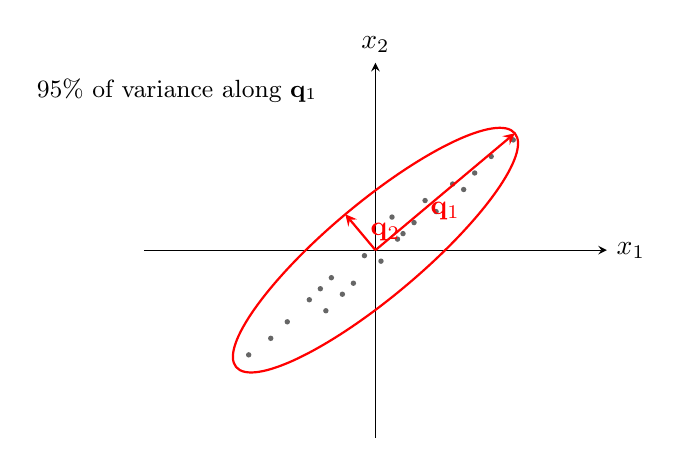
\begin{tikzpicture}[scale=0.7,>=stealth]
\draw[->] (-4.2,0)--(4.2,0) node[right]{$x_1$};
\draw[->] (0,-3.4)--(0,3.4) node[above]{$x_2$};
% scattered correlated data
\foreach \p in {(0.5,0.3),(-0.8,-0.5),(1.4,1.2),(-1.6,-1.3),(0.9,0.9),(-0.2,-0.1),(2.1,1.7),(-0.6,-0.8),(1.1,0.7),(-2.3,-1.9),(0.3,0.6),(-1.2,-0.9),(1.8,1.4),(-0.4,-0.6),(0.7,0.5),(-1.9,-1.6),(1.6,1.1),(0.1,-0.2),(-1.0,-0.7),(2.5,2.0),(0.4,0.2),(-0.9,-1.1)} \fill[black!60] \p circle (1.4pt);
\begin{scope}[rotate=40]
\draw[red,thick] (0,0) ellipse (3.3 and 0.85);
\draw[->,thick,red] (0,0)--(3.3,0) node[midway,below]{$\mathbf q_1$};
\draw[->,thick,red] (0,0)--(0,0.85) node[midway,right]{$\mathbf q_2$};
\end{scope}
\node at (-3.6,2.9) {\small 95\% of variance along $\mathbf q_1$};
\end{tikzpicture}

\caption{Covariance ellipse on real-ish data. Notice the ellipse's long
axis is the eigenvector of the largest eigenvalue --- that IS the
principal component, and its length is the eigenvalue's square root.
Regenerate: \ttfamily figures/ch09\_covellipse.tex.}
\label{fig:covellipse}
\end{figure}

\begin{lstlisting}[caption={\ttfamily code/ch09\_covariance.py --- PCA
directions fall straight out of \ttfamily np.linalg.eigh on the
covariance matrix.}]
import numpy as np
np.set_printoptions(precision=4, suppress=True)

# correlated 2-D data: x1 height-ish, x2 = 0.8 x1 + noise
rng = np.random.default_rng(4)
n = 400
x1 = rng.standard_normal(n)
x2 = 0.8 * x1 + 0.4 * rng.standard_normal(n)
X = np.column_stack([x1, x2])
X = X - X.mean(axis=0)
C = X.T @ X / (n - 1)
print("covariance C ="); print(C)
w, Q = np.linalg.eigh(C)
order = np.argsort(w)[::-1]
w, Q = w[order], Q[:, order]
print("eigenvalues:", w)
print("eigenvectors (cols):"); print(Q)
var_frac = w / w.sum()
print("variance fraction:", var_frac)
proj = X @ Q[:, 0]
print("reconstruction error keeping PC1:",
      np.mean((X - np.outer(proj, Q[:, 0]))**2))
print("PC1 direction angle (deg):", np.degrees(np.arctan2(Q[1,0], Q[0,0])))
\end{lstlisting}

\begin{lstlisting}[caption={Output of the covariance eigensolve. Notice
$95\%$ of variance rides one eigenvector --- projecting onto it loses
only $0.046$ mean-square error. This is chapter 10's PCA with the SVD
training wheels still on.}]
covariance C =
[[1.0254 0.8595]
 [0.8595 0.8843]]
eigenvalues: [1.8173 0.0925]
eigenvectors (cols):
[[-0.7355  0.6776]
 [-0.6776 -0.7355]]
variance fraction: [0.9516 0.0484]
reconstruction error keeping PC1: 0.046111017868167695
PC1 direction angle (deg): -137.34564252667914
\end{lstlisting}

\begin{figure}[htbp]
\centering
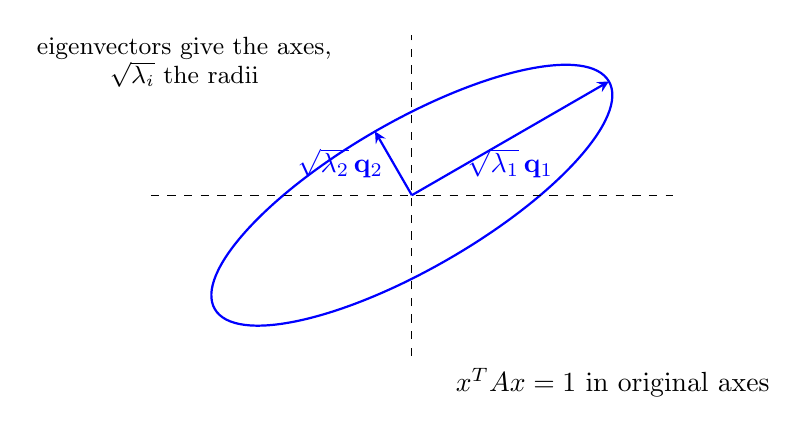
\begin{tikzpicture}[scale=0.85,>=stealth]
\begin{scope}[rotate=30]
\draw[blue,thick] (0,0) ellipse (3.4 and 1.1);
\draw[->,thick,blue] (0,0)--(3.4,0) node[midway,below]{$\sqrt{\lambda_1}\,\mathbf q_1$};
\draw[->,thick,blue] (0,0)--(0,1.1) node[midway,left]{$\sqrt{\lambda_2}\,\mathbf q_2$};
\end{scope}
\draw[dashed] (-3.9,0)--(3.9,0); \draw[dashed] (0,-2.4)--(0,2.4);
\node at (3.0,-2.8) {$x^{T}Ax=1$ in original axes};
\node at (-3.4,2.2) {\small eigenvectors give the axes,};
\node at (-3.4,1.8) {\small $\sqrt{\lambda_i}$ the radii};
\end{tikzpicture}

\caption{$x^{T}Ax=1$ is an ellipsoid whose axes are eigenvectors with
radii $1/\sqrt{\lambda_i}$ (for the form) --- or $\sqrt{\lambda_i}$ for
the covariance ellipsoid. Either way: eigenvectors are directions,
eigenvalues are lengths. Regenerate:
\ttfamily figures/ch09\_ellipsoid.tex.}
\label{fig:ellipsoid}
\end{figure}

\begin{exercise}[easy]
Why can no covariance matrix be indefinite?
\begin{solution}
$C=X^{T}X/(n-1)$ is a Gram matrix: $\mathbf v^{T}C\mathbf v=
\lVert X\mathbf v\rVert^{2}/(n-1)\ge0$ --- PSD by construction.
\end{solution}
\end{exercise}

\section{Hand derivation}\label{sec:handderiv9}

\textbf{Real eigenvalues.} Suppose $A=A^{T}$ real and
$A\mathbf v=\lambda\mathbf v$ with $\mathbf v\ne\mathbf0$ complex. Take
conjugate-transposes twice. First,
$\mathbf v^{*}A\mathbf v=\lambda\,\mathbf v^{*}\mathbf v$. Second,
conjugating the eigen equation: $A\bar{\mathbf v}=\bar\lambda\bar{\mathbf v}$
($A$ real), so
$\mathbf v^{*}A\mathbf v=(A^{T}\mathbf v)^{*}\mathbf v
=(A\mathbf v)^{*}\mathbf v$... directly:
$(\mathbf v^{*}A\mathbf v)^{*}=\mathbf v^{*}A^{T}\mathbf v
=\mathbf v^{*}A\mathbf v$ since $A=A^{T}$ --- the scalar
$\mathbf v^{*}A\mathbf v$ equals its own conjugate, hence real. But
$\mathbf v^{*}\mathbf v=\lVert\mathbf v\rVert^{2}>0$ is real and positive,
so $\lambda=\mathbf v^{*}A\mathbf v/\mathbf v^{*}\mathbf v$ is real.
\qed

\textbf{Orthogonal eigenvectors.} Let $A\mathbf v_1=\lambda_1\mathbf v_1$,
$A\mathbf v_2=\lambda_2\mathbf v_2$ with $\lambda_1\ne\lambda_2$. Then
\[
\lambda_1\,\mathbf v_1^{T}\mathbf v_2
=(A\mathbf v_1)^{T}\mathbf v_2
=\mathbf v_1^{T}A^{T}\mathbf v_2
=\mathbf v_1^{T}A\mathbf v_2
=\lambda_2\,\mathbf v_1^{T}\mathbf v_2,
\]
so $(\lambda_1-\lambda_2)\,\mathbf v_1^{T}\mathbf v_2=0$ and
$\mathbf v_1^{T}\mathbf v_2=0$. \qed

Together: eigenvalues real, and eigenvectors of distinct eigenvalues
orthogonal; repeated eigenvalues get orthonormalized inside their
eigenspace (Gram--Schmidt, ch.5), giving $Q$.

\section{Common mistakes}

\begin{tripwire}[{``Real matrix $\Rightarrow$ real eigenvalues''}]
False in general --- rotations have $\pm i$. The theorem is only for
symmetric $A$. Keep the hypothesis attached: $A^{T}=A$ is doing all the
work.
\end{tripwire}

\begin{tripwire}[{PSD vs.\ PD vs.\ indefinite confusion}]
$\ge0$ and $>0$ are different universes: PSD permits flat directions
($\lambda=0$), PD doesn't. Check $\lambda_{\min}=0$ before calling a
matrix PD --- and remember symmetric does NOT imply positive definite
($\begin{bmatrix}1&2\\2&1\end{bmatrix}$ is symmetric and indefinite).
\end{tripwire}

\begin{tripwire}[{Believing $A^{T}A$ can be negative definite}]
$\mathbf x^{T}A^{T}A\mathbf x=\lVert A\mathbf x\rVert^{2}\ge0$ always ---
it cannot even have a negative eigenvalue. If your Gram matrix shows one,
the computation is wrong, not the theorem.
\end{tripwire}

\begin{tripwire}[{Mixing up similarity with orthogonal similarity}]
$B=P^{-1}AP$ shares eigenvalues only; $B=Q^{T}AQ$ additionally preserves
symmetry \emph{and} is perfectly conditioned. The spectral theorem is
orthogonal similarity --- don't reach for a general $P$ when $Q$ exists.
\end{tripwire}

\section{Summary}

\begin{center}
\begin{tabularx}{\textwidth}{l>{\raggedright\arraybackslash}X}
\toprule
\textbf{Object} & \textbf{What you need to know}\\
\midrule
Spectral theorem & $A=A^{T}\Rightarrow A=Q\Lambda Q^{T}$, $Q$ orthogonal,
$\Lambda$ real \\
Definiteness & PD: $\lambda_i>0$ / all pivots $>0$ / minors $>0$; PSD:
$\lambda_i\ge0$; indefinite: mixed signs \\
Gram matrices & $A^{T}A$ always PSD; PD iff full column rank \\
Rayleigh quotient & $R(x)=x^{T}Ax/x^{T}x\in[\lambda_n,\lambda_1]$;
extremes at eigenvectors (min--max) \\
Ellipsoids & eigenvectors $=$ axes, $\sqrt{\lambda_i}=$ radii \\
Covariance & PSD by construction; top eigenvector $=$ PC1 (PCA next
chapter) \\
\bottomrule
\end{tabularx}
\end{center}
\begin{rulebox}[{Watch instead}]
\begin{enumerate}
\item \emph{Symmetric Matrices and Positive Definiteness} --- MIT
OpenCourseWare, 18.06 Lecture 25, 43:52,
\url{https://youtu.be/UCc9q_cAhho} --- the spectral theorem plus the
definiteness tests, \S\ref{sec:spectral}--\S\ref{sec:quadform}
(accessed 2026-10-11).
\item \emph{Positive Definite Matrices and Minima} --- MIT
OpenCourseWare, 18.06 Lecture 27, 50:40,
\url{https://youtu.be/vF7eyJ2g3kU} --- definiteness as the second-
derivative test, \S\ref{sec:quadform} (accessed 2026-10-11).
\end{enumerate}
\end{rulebox}

\section*{Further reading}
\addcontentsline{toc}{section}{Further reading}

\begin{itemize}
\item G.~Strang, \emph{Introduction to Linear Algebra}, 6th ed., \S6.4
(textbook level) --- symmetric matrices and the spectral theorem.
\item MIT OpenCourseWare, \emph{18.06SC Linear Algebra}, Unit III ---
recitations on positive definiteness, at OCW (course ``18.06SC'',
Unit III page ``Positive definite matrices''), at
\url{https://ocw.mit.edu}. Verified 2026-10-11.
\item Margalit and Rabinoff, \emph{Interactive Linear Algebra},
``The Spectral Theorem'' --- orthonormal diagonalization with more
examples. \newline
\url{https://textbooks.math.gatech.edu/ila/}
Verified 2026-10-11.
\item S.~Boyd and L.~Vandenberghe, \emph{VMLS}, \S8.3 (free PDF) ---
quadratic forms in the data register.\newline
\url{https://web.stanford.edu/~boyd/vmls/vmls.pdf}
Verified 2026-10-11.
\item M.~Deisenroth et al., \emph{Mathematics for Machine Learning},
\S3.5 (free PDF) --- symmetric positive-definite matrices for ML
kernels and metrics.\newline
\url{https://mml-book.github.io/book/mml-book.pdf}
Verified 2026-10-11.
\end{itemize}

\section*{Additional exercises}
\addcontentsline{toc}{section}{Additional exercises}

\begin{exercise}[easy]
Decide whether each is symmetric: $A+A^{T}$, $A-A^{T}$, $A^{T}A$,
$AA^{T}$, $ABA^{T}$ with $B$ symmetric.
\end{exercise}

\begin{exercise}[easy]
Classify definiteness of $\begin{bmatrix}2&0\\0&3\end{bmatrix}$,
$\begin{bmatrix}0&1\\1&0\end{bmatrix}$,
$\begin{bmatrix}1&1\\1&1\end{bmatrix}$ from their eigenvalues.
\end{exercise}

\begin{exercise}[easy]
Give a symmetric matrix with eigenvalues $4$ and $-2$, and one with $4$
and $0$. Which is invertible?
\end{exercise}

\begin{exercise}[easy]
Compute $R(\mathbf x)$ for $A=\operatorname{diag}(5,1)$ at
$\mathbf x=(1,0),(0,1),(1,1)$. Where do max/min sit?
\end{exercise}

\begin{exercise}[medium]
Show that $A$ PD and $B$ PD implies $A+B$ PD. Does $AB$ stay symmetric?
Give a counterexample or proof.
\end{exercise}

\begin{exercise}[medium]
Classify definiteness of
$\begin{bmatrix}4&2&0\\2&4&0\\0&0&-1\end{bmatrix}$ two ways (pivots,
eigenvalues) without a computer.
\end{exercise}

\begin{exercise}[medium]
Show that if $A$ is PSD then its diagonal entries are $\ge0$, and
$a_{ii}=0$ forces the entire row/column $i$ to be zero. (Hint: test
vectors $\mathbf e_i$ and $\mathbf e_i+t\mathbf e_j$.)
\end{exercise}

\begin{exercise}[medium]
In code: generate a $3\times3$ symmetric $A$, compute $R(\mathbf x)$ on
100 random unit vectors, and show the empirical max/min approximate
$\lambda_1,\lambda_3$ --- then locate the maximizer closest to the top
eigenvector.
\end{exercise}

\begin{exercise}[medium]
The Hessian of $f(x,y)=x^{2}+4xy+y^{2}$ is constant. Classify the
critical point at the origin by definiteness.
\end{exercise}

\begin{exercise}[hard]
Prove the min--max principle: $\lambda_k$ equals the maximum of
$R(\mathbf x)$ over the subspace orthogonal to
$\mathbf q_1,\dots,\mathbf q_{k-1}$, and every maximizer is an
eigenvector for $\lambda_k$.
\end{exercise}

\begin{exercise}[hard]
Show $A$ PD $\Rightarrow$ there is a unique PSD ``square root''
$A^{1/2}=Q\Lambda^{1/2}Q^{T}$ with $A^{1/2}A^{1/2}=A$, and use it to
explain the covariance-ellipsoid radii.
\end{exercise}

\begin{exercise}[hard]
Interlacing: prove that deleting the last row and column of a symmetric
$A$ interlaces the eigenvalues,
$\lambda_1(A)\ge\lambda_1(A')\ge\lambda_2(A)\ge\cdots\ge\lambda_{n-1}(A')
\ge\lambda_n(A)$. (Rayleigh quotient over a subspace does all the work.)
\end{exercise}
\begin{exercise}[easy]
For $A=\begin{bmatrix}3&0\\0&1\end{bmatrix}$, sketch the level set
$\mathbf{x}^{T}A\mathbf{x}=3$ and name it. Which axis is shorter, and
why does that match the bigger eigenvalue?
\end{exercise}
\begin{exercise}[medium]
Compute the Rayleigh quotient of
$A=\begin{bmatrix}2&1\\1&2\end{bmatrix}$ on $(2,0)$ and on
$(\cos\theta,\sin\theta)$ as a function of $\theta$; find its maximum
over $\theta$ and confirm it is $\lambda_{\max}$.
\end{exercise}
\begin{exercise}[hard]
Prove the max principle: a symmetric $A$ with eigenvalues
$\lambda_1\geq\cdots\geq\lambda_n$ satisfies
$\max_{\|\mathbf{x}\|=1}\mathbf{x}^{T}A\mathbf{x}=\lambda_1$.
(Hint: write $\mathbf{x}$ in the eigenbasis and bound each term.)
\end{exercise}

\chapternotes{%
The rotate--stretch--rotate framing and definiteness-via-pivots follow
Strang \cite{ila} and 18.06SC Unit III \cite{ocw1806sc}; Axler ch.~7
\cite{axler} gives the cleaner operator-theory route (self-adjoint first,
eigenvalues as a consequence); MML \S3.5 and ch.~4 \cite{mml} anchor the
PSD/quadratic-form clarity we borrow (its issue tracker documents exactly
the PD/PSD confusion we tripwire). The covariance-as-PSD application
follows VMLS \cite{vmls}; PCA proper arrives next chapter.}
